%%%%%%%%%%%%%%%%%%%%%%%%%%%%%%%%%%%%%%%%%%%%%%%%%%%%%%%%%%%%%%%%%%%%%%%%%%%%%%%%%%%%
%Do not alter this block of commands.  If you're proficient at LaTeX, you may include additional packages, create macros, etc. immediately below this block of commands, but make sure to NOT alter the header, margin, and comment settings here. 
\documentclass[12pt]{article}
 \usepackage[margin=1in]{geometry} 
\usepackage{amsmath,amsthm,amssymb,amsfonts, enumitem, fancyhdr, color, comment, graphicx, environ}
\pagestyle{fancy}
\setlength{\headheight}{65pt}
\newenvironment{problem}[2][Problem]{\begin{trivlist}
\item[\hskip \labelsep {\bfseries #1}\hskip \labelsep {\bfseries #2.}]}{\end{trivlist}}
\newenvironment{sol}
    {\emph{Solution:}
    }
    {
    \qed
    }
\specialcomment{com}{ \color{blue} \textbf{Comment:} }{\color{black}} %for instructor comments while grading
\NewEnviron{probscore}{\marginpar{ \color{blue} \tiny Problem Score: \BODY \color{black} }}
%%%%%%%%%%%%%%%%%%%%%%%%%%%%%%%%%%%%%%%%%%%%%%%%%%%%%%%%%%%%%%%%%%%%%%%%%%%%%%%%%

\usepackage{tabto}
\usepackage{tikz}
\usepackage{tkz-berge}

%%%%%%%%%%%%%%%%%%%%%%%%%%%%%%%%%%%%%%%%%%%%%
%Fill in the appropriate information below
\lhead{Chenhao WU \\ 117010285}  %replace with your name
\rhead{Networks: Techonology, Economics and Society\\ EIE3280 Summer 2019 \\ Assignment 1} %replace XYZ with the homework course number, semester (e.g. ``Spring 2019"), and assignment number.
%%%%%%%%%%%%%%%%%%%%%%%%%%%%%%%%%%%%%%%%%%%%%

\begin{document}
\begin{problem}{1}	
	(a) Consider 3 pairs of transmitters and receivers in a cell, with the following channel gain matrix \textbf{G} and noise of 0.1 mW for all the receivers. The target SIRs are shown below. With an initialization of all transmit powers at 1mW, run DPC for 10 iterations and plot the evolution of transmit powers and of received SIRs.\\
	You can use any programming language to calculate, or even write the steps out by hand. Please turn in the code or all the hand-written steps, respectively.
	$$	
	\textbf{G} = \begin{pmatrix}1 & 0.1 & 0.3\\0.2 & 1 & 0.3\\ 0.2 & 0.2 & 1 \\\end{pmatrix}, \gamma = \begin{pmatrix}
	1 \\ 1.5 \\ 1\\
	\end{pmatrix}
	$$
	\\
	(b) Now suppose the power levels for logical links 1, 2, 3 have converged as in the previous problem. A new pair of transmitter and receiver, labeled as logical link 4, shows up in the same cell, with an initial transmit power of 1 mW and demands a target SIR of 1. The new channel gain matrix is shown below. Similar to what you did for Problem 1 above, show what happens in the next 10 timeslots? What happens at the new equilibrium?
	$$
	\textbf{G} = \begin{pmatrix}
	 1 & 0.1 & 0.3 & 0.1 \\ 0.2 & 1 & 0.3 & 0.1 \\ 0.2 & 0.2 & 1 & 0.1 \\ 0.1 & 0.1 & 0.1 & 1\\
	\end{pmatrix}
	$$
\end{problem}
\begin{sol}
	Based on the computer simulation, we obtain following plots for question (a) and (b): \\
	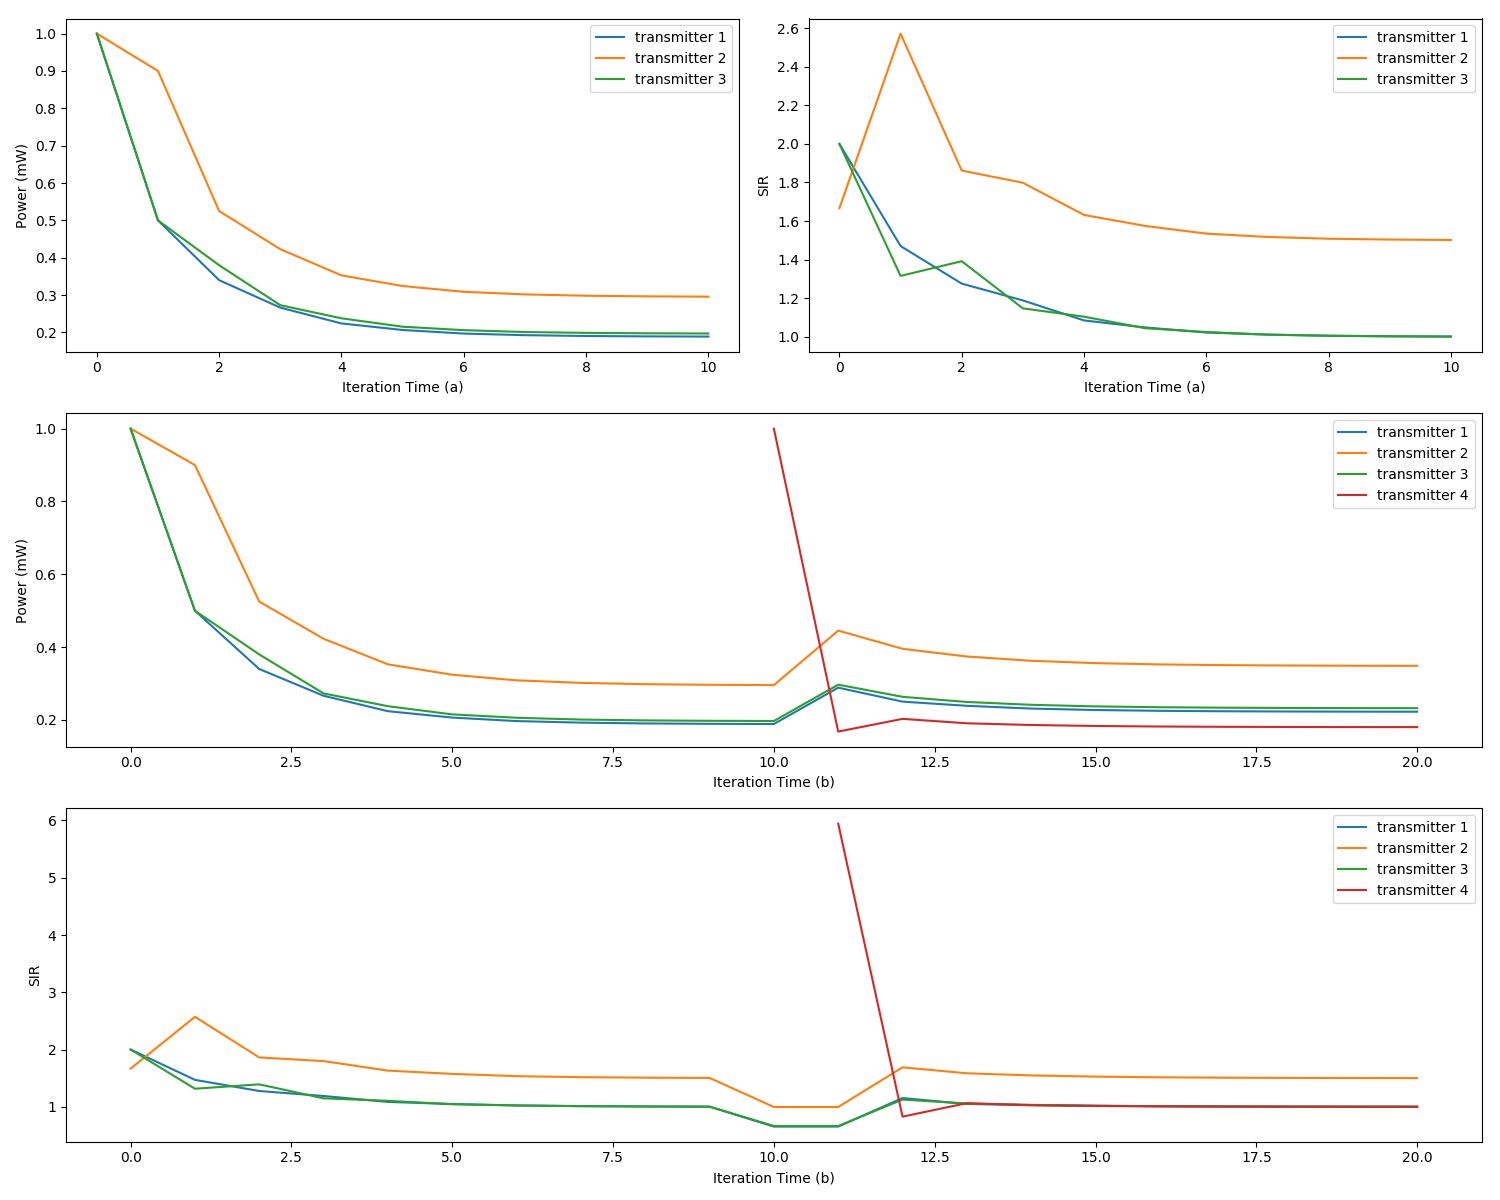
\includegraphics[width=\linewidth, height=0.5\textheight]{../assets/myplot.png}\\
	To answer the question (b), we find that after adding link 4 into the cell the transmission powers of other links at the equilibrium point have been raised, suggesting that the participation of link 4 brings interference to the other link, such that other links have to raise their transmission power in order to achieve the target SIRs. \\
	\textit{(Attachment: src/problem\_1\_1.py)}
\end{sol}

\begin{problem}{2}
	Three advertisers, 1, 2, and 3, bid for two ad spaces A, B. The average avenue of per click are \$6, \$4, \$3 for the bidders respectively, and the click through rate of the ad spaces are 500, 300 clicks per hour respectively.  \\
	(a) Draw the bipartite graph with nodes indicating advertisers or ad spaces and edges indicating values per hour. Indicate the maximum matching with bold lines. \\
	(b) What is the result of the GSP auction, assuming truthful bidding: allocation, prices changed, and payoffs received? \\
\end{problem}
\begin{sol}
	(a) From given conditions, we can obtain a bipartite graph as following \\
	\begin{tikzpicture}[shorten >=1pt, auto, node distance=3cm, thick,
	node_style/.style={circle,draw,font=\sffamily\Large\bfseries, minimum width=60pt},
	edge_style/.style={draw=black},
	bold_edge_style/.style={draw=black, line width=4pt}]
	\node[node_style] (a1) at (-4, 4) [text width=50pt, align=center]{\footnotesize Advertiser 1};
	\node[node_style] (a2) at (-4, 0) [text width=50pt, align=center]{\footnotesize Advertiser 2};
	\node[node_style] (a3) at (-4, -4) [text width=50pt, align=center]{\footnotesize Advertiser 3};
	\node[node_style] (b1) at (4, 4) [text width=50pt, align=center]{\footnotesize Ad Space 1};
	\node[node_style] (b2) at (4, 0) [text width=50pt, align=center]{\footnotesize Ad Space 2};
	\draw[bold_edge_style] (a1) edge node [xshift=-40]{3000\$/hour} (b1);
	\draw[edge_style] (a1) edge node [xshift=-72,yshift=30]{1800\$/hour} (b2);
	\draw[edge_style] (a2) edge node [xshift=-5,yshift=-20]{2000\$/hour} (b1);
	\draw[bold_edge_style] (a2) edge node [xshift=-40]{1200\$/hour} (b2);
	\draw[edge_style] (a3) edge node [xshift=-5,yshift=-50]{1500\$/hour} (b1);
	\draw[edge_style] (a3) edge node [xshift=-5,yshift=-50]{900\$/hour} (b2);
	\end{tikzpicture}\\
	(b) According the GSP mechanism, the result of auction can be derived as that, the Ad space 1 is allocated to Advertiser 1 with a price of 3000\$/hour, and the Ad space 2 is allocated to Advertiser 2 with a price of 1200\$/hour. The payoffs of both these three advertisers are zero.
\end{sol}

\begin{problem}{3}
	Tom and Jimmy are bidding for three ad slots on a page, and one bidder can win at most one slot. Suppose an ad in the first slot receives 500 clicks per hour, while the second and third slot get 300, 200 clicks per hour respectively. Assume Tom receive $r$ value per click. \\
	(a) Denote by $b, b^\prime$ as the bids by Tom and Jimmy respectively. In GSP auction, discuss Tom's payoff $ f $ in terms of $ b, b^\prime $.\\
	(b) Does Tom have a dominant strategy?
\end{problem}
\begin{sol}
	(a) According to given conditions we can obtain that Tom's hourly revenue received in ad slot 1, 2 and 3 are $500r$, $300r$ and $200r$ respectively. Assume that both two bids are truthful bidding, then for Tom's bidding $b$ we have 
	\begin{align*}
		b &= \begin{pmatrix}
		500r \\ 300r \\ 200r \\
		\end{pmatrix}
	\end{align*}
	\textbf{i.} \textit{If $b_1 > b_1^\prime$}, then Jimmy wins the first slot, then the payoff of Tom is $f = 300r - b_2^\prime$. \\
	\textbf{ii.} \textit{If $b_1 < b_1^\prime$}, then Tom wins the first slot, then the payoff of Tom equals to 0.\\
	(b). There is not a dominant strategy in GSP auction. The direct reason contribute to this conclusion is that \textit{Truth-telling is not a dominant strategy for GSP}, and for many cases we can show the statement holds. If we look inside the GSP auction, it is easy to find that unlike in the second price auction there is a agent that internalizes the externality damage from the winner to the other, in GSP the externality damage from the winner can not be internalized, thus there is not a equilibrium for players in a GSP auction. If the auction is converted to a VCG auction, in which the externality damage can be eliminated, then we can discuss the dominant strategy and the nash equilibrium. 
\end{sol}
\end{document}